\section{Methodik}
\label{sec:methodik}

Die vorliegende Bachelorarbeit beschäftigt sich mit der Dekodierung verschiedener Dreiecksnetze mittels dem Kodierungstandard Brotli-G.
Diese Methodiksektion dient dazu, einen detaillierten Einblick auf die Durchführung und Analyse des Experiments zu geben.
Das Experiment zielt darauf ab, komprimierte Dreiecksnetze auf der GPU zu dekomprimieren.
Insbesondere sollen das Kompressionsverhältnis, Dekompressionsgeschwindigkeit und die visualle Qualität quantitativ ausgewertet werden.

\subsection{Ablauf des Experiments}
\label{subsec:ablauf}
Zu Beginn muss der Datensatz mittels Brotli-G kodiert werden.
Der Einfachheit halber wird in diesem Abschnitt von einem einzigen Dreiecksnetz gesprochen.
Der Meshoptimizer von Zeux \cite{Zeux} ist dafür verantwortlich, aus den Positionen und Indizes die Meshletdaten zu generieren.
Dazu wurde ein Binärformat entworfen, das die relevanten Daten zum Darstellen des gesamten Dreiecksnetzes speichert.
Das Binärformat besteht dementsprechend aus dem Meshlet Descriptor, Vertex Ressourcen (Positionen und Normalen) und den Indizes zur Primitivengenerierung.
Das Binärformat wird anschließend als gesamtes komprimiert.
Anschließend werden die GPU Resourcen für die Eingabe (komprimiertes Dreiecksnetz) und Ausgabe (dekomprimiertes Dreiecksnetz) angelegt.
Für die Ausgabe wird eine \glqq Unordered Acces View (UAV)\grqq\ verwendet.
Wie der Name schon vermuten lässt, bietet diese eine flexiblere Möglichkeit, gleichzeitig an verschiedenen Orten zu lesen und schreiben.
Besonders von Vorteil ist dieser Ressourcentyp für die parellele Verarbeitung.
So können einzelne Threads von der Ressource lesen/schreiben, ohne darauf warten zu müssen, bis ein anderer Thread die Ressource wieder freigibt.

\begin{figure}[htb]
  \centering  
  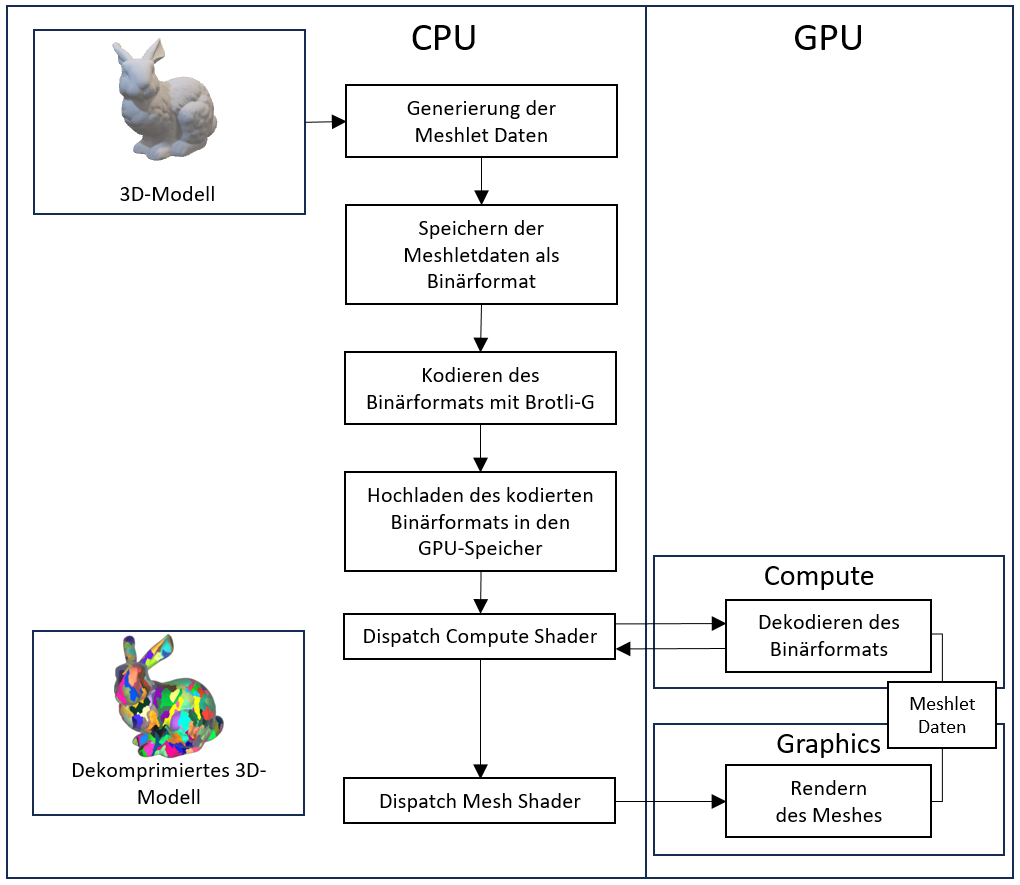
\includegraphics[scale=0.6]{Bilder/Ablauf_Projekt.png}
  \caption[Flussdiagramm Ablauf]{\textbf{Flussdiagramm Ablauf} Abbildung der Dekompressionspipeline.}
  \label{fig:projekt}
\end{figure}